\chapter{Übungsblatt 6}

\section{Aufgabe 1}

\subsection{a}
In der Vorlesung wurde behauptet, dass die Binomalverteilung viel mit der Bernouilli-Verteilung zu tun hat. Sortieren Sie für sich selbst: wie hängen die beiden genau zusammen?

Die Bernouilli-Verteilung ist ein einmaliger Zufallsversuch, die Bino\-mial\-verteilung betrachtet $n$ Zufallsversuche

\subsection{b}
Zeichnen Sie das Stäbchendiagramm zu $B(5,\frac{1}{6})$

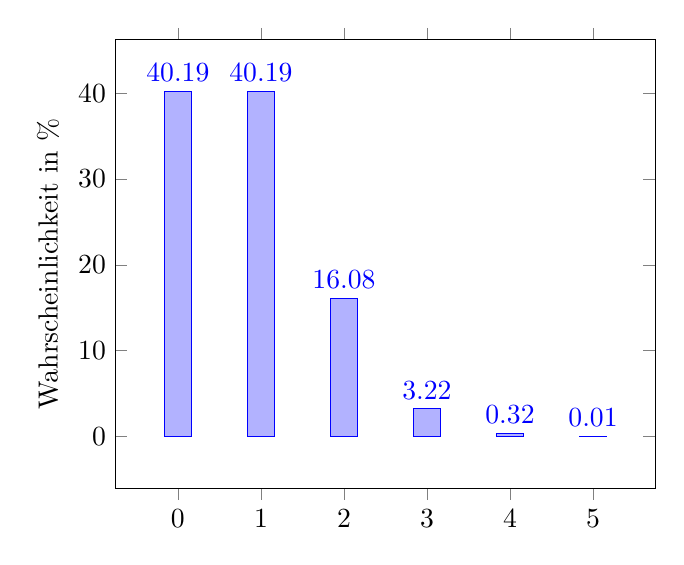
\begin{tikzpicture}
    \begin{axis}[
        ybar,
        enlargelimits=0.15,
        ylabel={Wahrscheinlichkeit in \%},
        symbolic x coords={0, 1, 2, 3, 4, 5},
        xtick=data,
        nodes near coords,
        nodes near coords align={vertical},
        /pgf/number format/fixed,
    ]
    \addplot coordinates {
        (0, 40.19)
        (1, 40.19)
        (2, 16.08)
        (3, 3.22) 
        (4, 0.32) 
        (5, 0.01) 
    };
    \end{axis}
\end{tikzpicture}

\section{Aufgabe 2}

\subsection{a}

Sie haben Geburtstag und Ihr Lieblingsonkel liebt seltsame Geschenke. Als Teil seines Geburtstagsgeschenks sollen Sie ein Spiel mit ihm spielen: sie müssen 10 Mal mit einem 12-seitigen Würfel würfeln. Würfeln Sie dabei mindestens 2 Mal den Monat Ihres Geburtstags, dann schenkt Ihr Onkel Ihnen ein neues Fahrrad. Wenn nicht, schenkt er Ihnen eine Tafel Schokolade. Wie groß ist die Wahrscheinlichkeit dafür, dass Sie ein Fahrrad bekommen?

\begin{align*}
    X = \text{"Anzahl gewürfelter Geburtsmonate"} \\
    X \sim B\left(n, p\right) \\
    X \sim B\left(10, \frac{1}{12}\right) \\
    P(X) = \begin{pmatrix}
        n \\ k
    \end{pmatrix} \cdot p^k \cdot {(1 - p)}^{n - k} \\
    P(X \geq 2) = 1 - \left(
        \begin{aligned}
            & \binom{10}{0} \cdot {\left(\frac{1}{12}\right)}^0 \cdot {\left(1 - \frac{1}{12}\right)}^{10-0} \\
            & + \binom{10}{1} \cdot {\left(\frac{1}{12}\right)}^1 \cdot {\left(1 - \frac{1}{12}\right)}^{10-1}
        \end{aligned}
    \right) \\
    P(X \geq 2) \approx 1 - \left(
        \begin{aligned}
            & 0.4189 \\
            & + 0.3808
        \end{aligned}
    \right) \\
    P(X \geq 2) \approx 1 - 0.7997 \\
    P(X \geq 2) \approx 0.2003 \\
    P(X \geq 2) \approx 20.03\%
\end{align*}

\subsection{b} 

In einer Pralinenschachtel sind 8 mit Marzipan und 8 mit Nougat gefüllte Pralinen, die von außen gleich aussehen, zufällig angeordnet. Sie entnehmen und verspeisen 5 Pralinen. Wie groß ist die Wahrscheinlichkeit dafür, dass alle 5 Pralinen mit Marzipan gefüllt sind?

\begin{align*}
    X = \text{"verspeisten pralinen mit Marzipan"} \\
    X \sim H\left(N, M, n\right) \\
    X \sim H\left(16,  8, 5\right) \\
    P(X) = \frac{\begin{pmatrix}
        M \\ k
    \end{pmatrix} \cdot \begin{pmatrix}
        N - M \\ n - k
    \end{pmatrix}}{\begin{pmatrix}
        N \\ n
    \end{pmatrix}} \\
    P(X = 5) = \frac{\begin{pmatrix}
        8 \\ 5
    \end{pmatrix} \cdot \begin{pmatrix}
        16 - 8 \\ 5 - 5
    \end{pmatrix}}{\begin{pmatrix}
        16 \\ 5
    \end{pmatrix}} \\
    P(X = 5) = \frac{\begin{pmatrix}
        8 \\ 5
    \end{pmatrix} \cdot \begin{pmatrix}
        8 \\ 0
    \end{pmatrix}}{\begin{pmatrix}
        16 \\ 5
    \end{pmatrix}} \\
    P(X = 5) = \frac{56\cdot 1}{4368} \\
    P(X = 5) = \frac{56}{4368} \\
    P(X = 5) = \frac{1}{78} \\
    P(X = 5) \approx 0.0128 \\
    P(X = 5) \approx 1.28\% \\
\end{align*}

\subsection{c}

Erinnern Sie sich an Max aus dem PIN-Beispiel (Foliensatz zu ST-K03, Seite 2 und 3)? Angenommen, er braucht 20 Sekunden, um eine PIN zu probieren. Wie groß ist (im Szenario von Seite 3) die Wahrscheinlichkeit dafür, dass der innerhalb von 5 Minuten die richtige PIN errät, wenn er sich merkt, welche PINs er bereits durchprobiert hat? Wie groß ist die Wahrscheinlichkeit, wenn er sich nicht merkt, welche Zahlenkombinationen er bereits durchprobiert hat?

